\documentclass{standalone}
\usepackage{tikz}
\usetikzlibrary{patterns, positioning}


\begin{document}
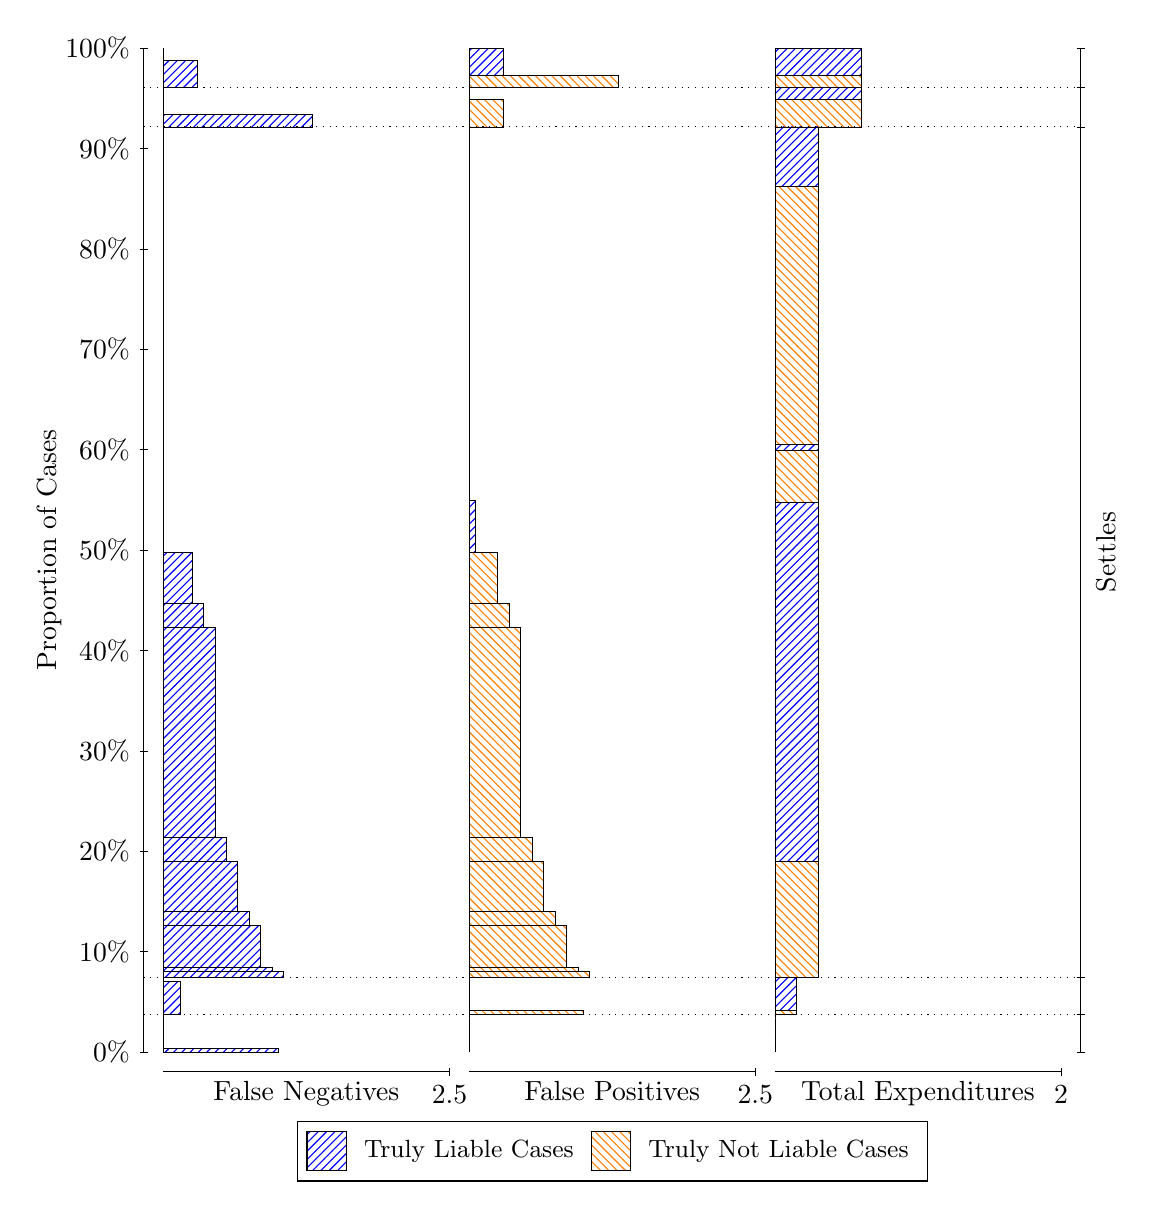
\begin{tikzpicture}
\draw[black, very thin] (1.5,1.75) -- (1.5,14.5);
\node[rotate=90, text=black, anchor=center] at (0.3, 8.125) {Proportion of Cases};
\draw[black, very thin] (1.45,1.75) -- (1.55,1.75);
\node[text=black, anchor=east] at (1.45, 1.75) {0\%};
\draw[black, very thin] (1.45,3.025) -- (1.55,3.025);
\node[text=black, anchor=east] at (1.45, 3.025) {10\%};
\draw[black, very thin] (1.45,4.3) -- (1.55,4.3);
\node[text=black, anchor=east] at (1.45, 4.3) {20\%};
\draw[black, very thin] (1.45,5.575) -- (1.55,5.575);
\node[text=black, anchor=east] at (1.45, 5.575) {30\%};
\draw[black, very thin] (1.45,6.85) -- (1.55,6.85);
\node[text=black, anchor=east] at (1.45, 6.85) {40\%};
\draw[black, very thin] (1.45,8.125) -- (1.55,8.125);
\node[text=black, anchor=east] at (1.45, 8.125) {50\%};
\draw[black, very thin] (1.45,9.4) -- (1.55,9.4);
\node[text=black, anchor=east] at (1.45, 9.4) {60\%};
\draw[black, very thin] (1.45,10.675) -- (1.55,10.675);
\node[text=black, anchor=east] at (1.45, 10.675) {70\%};
\draw[black, very thin] (1.45,11.95) -- (1.55,11.95);
\node[text=black, anchor=east] at (1.45, 11.95) {80\%};
\draw[black, very thin] (1.45,13.225) -- (1.55,13.225);
\node[text=black, anchor=east] at (1.45, 13.225) {90\%};
\draw[black, very thin] (1.45,14.5) -- (1.55,14.5);
\node[text=black, anchor=east] at (1.45, 14.5) {100\%};

\draw[black, very thin] (13.4,1.75) -- (13.4,14.5);
\draw[black, very thin] (13.35,1.75) -- (13.45,1.75);
\node[anchor=west] at (13.35, 1.75) {};
\draw[black, very thin] (13.35,2.2245) -- (13.45,2.2245);
\node[anchor=west] at (13.35, 2.2245) {};
\draw[black, very thin] (13.35,2.6989) -- (13.45,2.6989);
\node[anchor=west] at (13.35, 2.6989) {};
\draw[black, very thin] (13.35,13.499) -- (13.45,13.499);
\node[anchor=west] at (13.35, 13.499) {};
\draw[black, very thin] (13.35,13.999) -- (13.45,13.999);
\node[anchor=west] at (13.35, 13.999) {};
\draw[black, very thin] (13.35,14.5) -- (13.45,14.5);
\node[anchor=west] at (13.35, 14.5) {};

\draw[black, very thin, pattern color=blue, pattern=north east lines] (1.75,1.75) rectangle (3.2033,1.7999);
\draw[black, very thin, pattern color=orange, pattern=north west lines] (1.75,1.7999) rectangle (1.75,2.2245);
\draw[black, very thin, pattern color=blue, pattern=north east lines] (1.75,2.2245) rectangle (1.968,2.649);
\draw[black, very thin, pattern color=orange, pattern=north west lines] (1.75,2.649) rectangle (1.75,2.6989);
\draw[black, very thin, pattern color=blue, pattern=north east lines] (1.75,2.6989) rectangle (3.276,2.7767);
\draw[black, very thin, pattern color=blue, pattern=north east lines] (1.75,2.7767) rectangle (3.1307,2.8244);
\draw[black, very thin, pattern color=blue, pattern=north east lines] (1.75,2.8244) rectangle (2.9853,3.3609);
\draw[black, very thin, pattern color=blue, pattern=north east lines] (1.75,3.3609) rectangle (2.84,3.5352);
\draw[black, very thin, pattern color=blue, pattern=north east lines] (1.75,3.5352) rectangle (2.6947,4.17);
\draw[black, very thin, pattern color=blue, pattern=north east lines] (1.75,4.17) rectangle (2.5493,4.4731);
\draw[black, very thin, pattern color=blue, pattern=north east lines] (1.75,4.4731) rectangle (2.404,7.1442);
\draw[black, very thin, pattern color=blue, pattern=north east lines] (1.75,7.1442) rectangle (2.2587,7.446);
\draw[black, very thin, pattern color=blue, pattern=north east lines] (1.75,7.446) rectangle (2.1133,8.0988);
\draw[black, very thin, pattern color=orange, pattern=north west lines] (1.75,8.0988) rectangle (1.75,13.499);
\draw[black, very thin, pattern color=blue, pattern=north east lines] (1.75,13.499) rectangle (3.6393,13.654);
\draw[black, very thin, pattern color=orange, pattern=north west lines] (1.75,13.654) rectangle (1.75,13.999);
\draw[black, very thin, pattern color=blue, pattern=north east lines] (1.75,13.999) rectangle (2.186,14.344);
\draw[black, very thin, pattern color=orange, pattern=north west lines] (1.75,14.344) rectangle (1.75,14.5);
\draw[black, very thin, pattern color=orange, pattern=north west lines] (5.6333,1.75) rectangle (5.6333,2.1746);
\draw[black, very thin, pattern color=blue, pattern=north east lines] (5.6333,2.1746) rectangle (5.6333,2.2245);
\draw[black, very thin, pattern color=orange, pattern=north west lines] (5.6333,2.2245) rectangle (7.0867,2.2744);
\draw[black, very thin, pattern color=blue, pattern=north east lines] (5.6333,2.2744) rectangle (5.6333,2.6989);
\draw[black, very thin, pattern color=orange, pattern=north west lines] (5.6333,2.6989) rectangle (7.1593,2.7767);
\draw[black, very thin, pattern color=orange, pattern=north west lines] (5.6333,2.7767) rectangle (7.014,2.8244);
\draw[black, very thin, pattern color=orange, pattern=north west lines] (5.6333,2.8244) rectangle (6.8687,3.3608);
\draw[black, very thin, pattern color=orange, pattern=north west lines] (5.6333,3.3608) rectangle (6.7233,3.5352);
\draw[black, very thin, pattern color=orange, pattern=north west lines] (5.6333,3.5352) rectangle (6.578,4.17);
\draw[black, very thin, pattern color=orange, pattern=north west lines] (5.6333,4.17) rectangle (6.4327,4.4731);
\draw[black, very thin, pattern color=orange, pattern=north west lines] (5.6333,4.4731) rectangle (6.2873,7.1442);
\draw[black, very thin, pattern color=orange, pattern=north west lines] (5.6333,7.1442) rectangle (6.142,7.4461);
\draw[black, very thin, pattern color=orange, pattern=north west lines] (5.6333,7.4461) rectangle (5.9967,8.0989);
\draw[black, very thin, pattern color=blue, pattern=north east lines] (5.6333,8.0989) rectangle (5.706,8.7516);
\draw[black, very thin, pattern color=blue, pattern=north east lines] (5.6333,8.7516) rectangle (5.6333,13.499);
\draw[black, very thin, pattern color=orange, pattern=north west lines] (5.6333,13.499) rectangle (6.0693,13.844);
\draw[black, very thin, pattern color=blue, pattern=north east lines] (5.6333,13.844) rectangle (5.6333,13.999);
\draw[black, very thin, pattern color=orange, pattern=north west lines] (5.6333,13.999) rectangle (7.5227,14.155);
\draw[black, very thin, pattern color=blue, pattern=north east lines] (5.6333,14.155) rectangle (6.0693,14.5);
\draw[black, very thin, pattern color=orange, pattern=north west lines] (9.5167,1.75) rectangle (9.5167,2.1746);
\draw[black, very thin, pattern color=blue, pattern=north east lines] (9.5167,2.1746) rectangle (9.5167,2.2245);
\draw[black, very thin, pattern color=orange, pattern=north west lines] (9.5167,2.2245) rectangle (9.7892,2.2744);
\draw[black, very thin, pattern color=blue, pattern=north east lines] (9.5167,2.2744) rectangle (9.7892,2.6989);
\draw[black, very thin, pattern color=orange, pattern=north west lines] (9.5167,2.6989) rectangle (10.062,4.17);
\draw[black, very thin, pattern color=blue, pattern=north east lines] (9.5167,4.17) rectangle (10.062,8.7336);
\draw[black, very thin, pattern color=orange, pattern=north west lines] (9.5167,8.7336) rectangle (10.062,9.3863);
\draw[black, very thin, pattern color=blue, pattern=north east lines] (9.5167,9.3863) rectangle (10.062,9.4641);
\draw[black, very thin, pattern color=orange, pattern=north west lines] (9.5167,9.4641) rectangle (10.062,12.74);
\draw[black, very thin, pattern color=blue, pattern=north east lines] (9.5167,12.74) rectangle (10.062,13.499);
\draw[black, very thin, pattern color=orange, pattern=north west lines] (9.5167,13.499) rectangle (10.607,13.844);
\draw[black, very thin, pattern color=blue, pattern=north east lines] (9.5167,13.844) rectangle (10.607,13.999);
\draw[black, very thin, pattern color=orange, pattern=north west lines] (9.5167,13.999) rectangle (10.607,14.155);
\draw[black, very thin, pattern color=blue, pattern=north east lines] (9.5167,14.155) rectangle (10.607,14.5);
\draw[black, dotted] (1.5,2.2245) -- (13.4,2.2245);
\draw[black, dotted] (1.5,2.6989) -- (13.4,2.6989);
\draw[black, dotted] (1.5,13.499) -- (13.4,13.499);
\draw[black, dotted] (1.5,13.999) -- (13.4,13.999);
\draw[black, very thin] (1.75,1.5) -- (5.3833,1.5);
\node[text=black, anchor=north] at (3.5667, 1.5) {False Negatives};
\draw[black, very thin] (5.3833,1.45) -- (5.3833,1.55);
\node[text=black, anchor=north] at (5.3833, 1.45) {2.5};

\draw[black, very thin] (5.6333,1.5) -- (9.2667,1.5);
\node[text=black, anchor=north] at (7.45, 1.5) {False Positives};
\draw[black, very thin] (9.2667,1.45) -- (9.2667,1.55);
\node[text=black, anchor=north] at (9.2667, 1.45) {2.5};

\draw[black, very thin] (9.5167,1.5) -- (13.15,1.5);
\node[text=black, anchor=north] at (11.333, 1.5) {Total Expenditures};
\draw[black, very thin] (13.15,1.45) -- (13.15,1.55);
\node[text=black, anchor=north] at (13.15, 1.45) {2};



\node[text=black, centered, rotate=90] at (13.72, 8.0988) {Settles};



\draw (7.449999999999999,1.5) node[draw=none] (baseCoordinate) {};
\begin{scope}[align=center]
        \matrix[scale=0.5, draw=black, below=0.5cm of baseCoordinate, nodes={draw}, column sep=0.1cm]{
            \node[rectangle, draw, minimum width=0.5cm, minimum height=0.5cm, pattern color=blue, pattern=north east lines] {}; &
            \node[draw=none, font=\small, text=black] (B) {Truly Liable Cases}; &
            \node[rectangle, draw, minimum width=0.5cm, minimum height=0.5cm, pattern color=orange, pattern=north west lines] {}; &
            \node[draw=none, font=\small, text=black] (B) {Truly Not Liable Cases}; \\
            };
\end{scope}

\end{tikzpicture}
\end{document}